\section{Overzicht van het systeem}

\subsection{Het Systeem}

\begin{figure}[H]
	\centering
	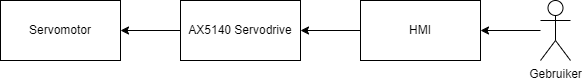
\includegraphics[width=\linewidth]{Systeemverband}
	\label{fig:SysteemVerband}
	\caption{Interfacing van gebruiker tot motor}
\end{figure}

In figuur \ref{fig:SysteemVerband} is de werking van het systeem te zien van de gebruiker tot de servomotor. De gebruiker kan via de \gls{HMI} de servodrive aansturen en daarmee dus ook de servomotor. De \gls{HMI} communiceert met de servodrive via \gls{EtherCAT} en \gls{SoE}. Standaard is dit \gls{EtherCAT} maar voor het schrijven en lezen van parameters gebruikt de drive \gls{SoE}.

\newpage

\subsection{Systeemcontext}

In figuur \ref{fig:Systeemcontext} is te zien waar de testkast gebruikt wordt. In eerste instantie wordt er een machine verkocht bij Voortman waar spindels in zitten voor het boren, tappen of vrezen van staal. Wanneer deze spindel na verloop van tijd niet meer correct functioneert wordt deze vervangen en wordt de kapotte spindel teruggestuurd richting Voortman. Hier wordt deze eventeel eerst getest als de oorzaak nog niet helemaal bekend is waarna de spindel gereviseerd wordt. Wanneer de spindel gereviseerd is zal deze nog getest worden om zeker te weten dat deze weer goed werkt waarna de spindel weer verkocht kan worden als gereviseerde spindel.

\begin{figure}[H]
	\centering
	\includegraphics[width=\linewidth]{Systeemcontext}
	\label{fig:Systeemcontext}
	\caption{Systeemcontext van de testkast}
\end{figure}

\newpage

\subsection{kritische analyse van de eisen}

In dit gedeelte van het functioneel ontwerp worden de belangrijkste eisen nog eens benoemd met daarbij de belangrijkste functies. Alle eisen staan gedefineerd in het SRD van de testkast (bijlage \ref{sec:TestKastSRD}). De focus van de opdracht zal liggen bij de volgende eisen in het \gls{SRD}:

\begin{itemize}
	\item \textbf{FR-001 Geautomatiseerd testen} Deze eis houdt in dat de testkast geautomatiseerd de spindel kan aftesten zonder dat hierbij iemand bij hoeft te zijn.
	\item \textbf{FR-006 Automatisch parameters inladen} Dit houdt in dat wanneer er een ander soort spindel op de testkast geladen wordt dat het programma op de testkast dan automatisch de bijpassende parameters kan inladen in de motordrive.
	\item \textbf{FR-007 Handmatig testen} Deze eis houdt in dat naast geautomatiseerd testen dat de gebruiker ook de mogelijkheid heeft om zelf de spindel te testen.
	\item \textbf{FR-009 Servo motoren} Deze eis houdt in dat de motordrive bepaalde motoren tenminste moet kunnen aansturen. Hier moet dus een parameterset van aanwezig zijn.
	\item \textbf{HR-004 Montage gaten} Dit houdt in dat de testkast de juiste gaten moet hebben op de montage plaat zodat alle spindels vastgemaakt kunnen worden aan de testkast.
\end{itemize} 

\newpage

\subsection{Functies}

Vermeld en beschreven hieronder zijn de functies die de testkast moet hebben, gebaseerd op de hoofdvragen en de eisen uit het \gls{SRD}. Er worden hier alleen functies beschreven die betrekking hebben op de opdracht. Bestaande functies die de testkast al heeft zijn al vervuld en zullen niet opnieuw worden gedefineerd.

\begin{enumerate}
	\item \textbf{Geautomatiseerd testen} De testkast moet in staat zijn om geautomatiseerd te testen zonder dat hier een operator voor nodig is.
	\item \textbf{Handmatig testen} Wanneer de gebruiker dit wil moet het ook mogelijk zijn om de spindel handmatig te testen dit betekend de spindel laten draaien op verschillende snelheden op basis van bijvoorbeeld een slider.
	\item \textbf{Automatisch de juiste parameters inladen} Wanneer er een andere gemonteerd wordt op de testkast moet het programma op de testkast automatisch de juiste parameters naar de drive schrijven. Dit betekend dat de gebruiker alleen hoeft te kiezen welke parameterset er naar de drive geschreven moeten worden.
	\item \textbf{Test onderbreking} In geval van een noodstop of bij het openen van de deuren van de testkast moet de testkast in noodstop gaan dit betekend dat alle bewegende delen moeten stoppen en dat het automatische testprogramma onderbroken wordt wanneer deze bezig is.
	\item \textbf{Toolchanger openen} Wanneer er op de \gls{gui} de toolchanger geopened wordt of op de toolchanger knop gedrukt wordt moet de toolchanger open gaan. Wanneer de toolchanger knop los gelaten wordt moet deze weer dicht gaan of wanneer er op de \gls{gui} op dicht gedrukt wordt.
	\item \textbf{Programma starten} Wanneer er op de startknop gedrukt wordt moet het testprogramma dat open staat beginnen.
	\item \textbf{Programma stoppen} Wanneer de stopknop ingedrukt wordt moet het testprogramma stoppen en ook moet de spindel stoppen mocht deze handmatig bediend zijn. Om weer te starten moet er eerst een reset zijn geweest.
	\item \textbf{Programma resetten} Wanneer de reset knop ingedrukt is moeten alle errors, warnings en messages in het programma gereset worden. Ook moet het weer mogelijk zijn om het programma te vervolgen of te starten.
\end{enumerate}

\newpage

\subsection{Functies overzicht}

De connecties tussen de functies zijn te zien in  figuur \ref{fig:TestkastInteractie}. Hierbij zal de meeste interactie via de \gls{gui} zijn echter is het wel mogelijk om de testkast te stoppen of om de toolchanger te openen met fysieke knoppen. Ook is er een reset knop aanwezig en een stop knop. Deze stopknop stopt niet heel het systeem maar alleen het programma dat aan het runnen kan zijn. Ook is er een start knop aanwezig waarmee het testprogramma gestart kan worden. Tot slot is er ook een reset knop aanwezig waarmee alle fouten in het programma gereset kunnen worden. Wanneer de reset knop ingedrukt is geweest moet het ook weer mogelijk zijn om het testprogramma te vervolgen.

\begin{figure}[H]
	\centering
	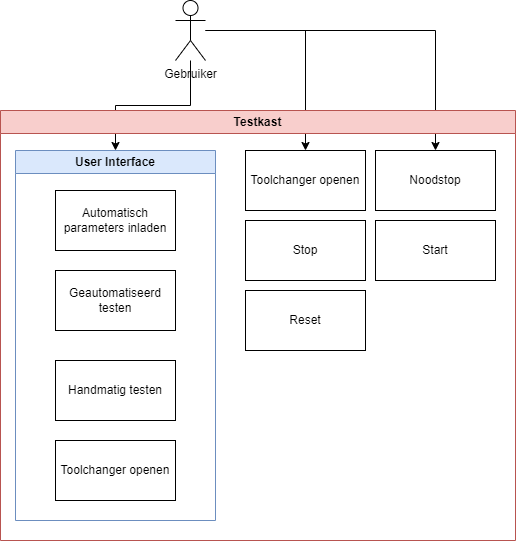
\includegraphics[width=0.8\linewidth]{TestkastInteractie}
	\label{fig:TestkastInteractie}
	\caption{Gebruiker interactie met het systeem}
\end{figure}